\documentclass[tikz,border=0pt]{standalone}
\usepackage{fontspec}
\hyphenpenalty=10000
\exhyphenpenalty=10000
\setmainfont[Path=../fonts/,BoldFont=Poppins-SemiBold.ttf,ItalicFont=Poppins-Italic.ttf]{Poppins-Regular.ttf}
\usepackage{pgfplots}
\pgfplotsset{compat=1.18}
\usetikzlibrary{calc,arrows.meta}
\definecolor{ink}{HTML}{161b22}
\definecolor{text}{HTML}{353535}
\definecolor{muted}{HTML}{646c74}
\definecolor{line}{HTML}{d7dadd}
\definecolor{wash}{HTML}{f6f6f6}
\definecolor{tint}{HTML}{e6ecef}
\definecolor{link}{HTML}{1d63b7}
\definecolor{local}{HTML}{376c97}
\definecolor{api}{HTML}{995d46}
\definecolor{cloud}{HTML}{7b649b}
\definecolor{match}{HTML}{7d9fc4}
\definecolor{miss}{HTML}{e0e3e5}
\begin{document}
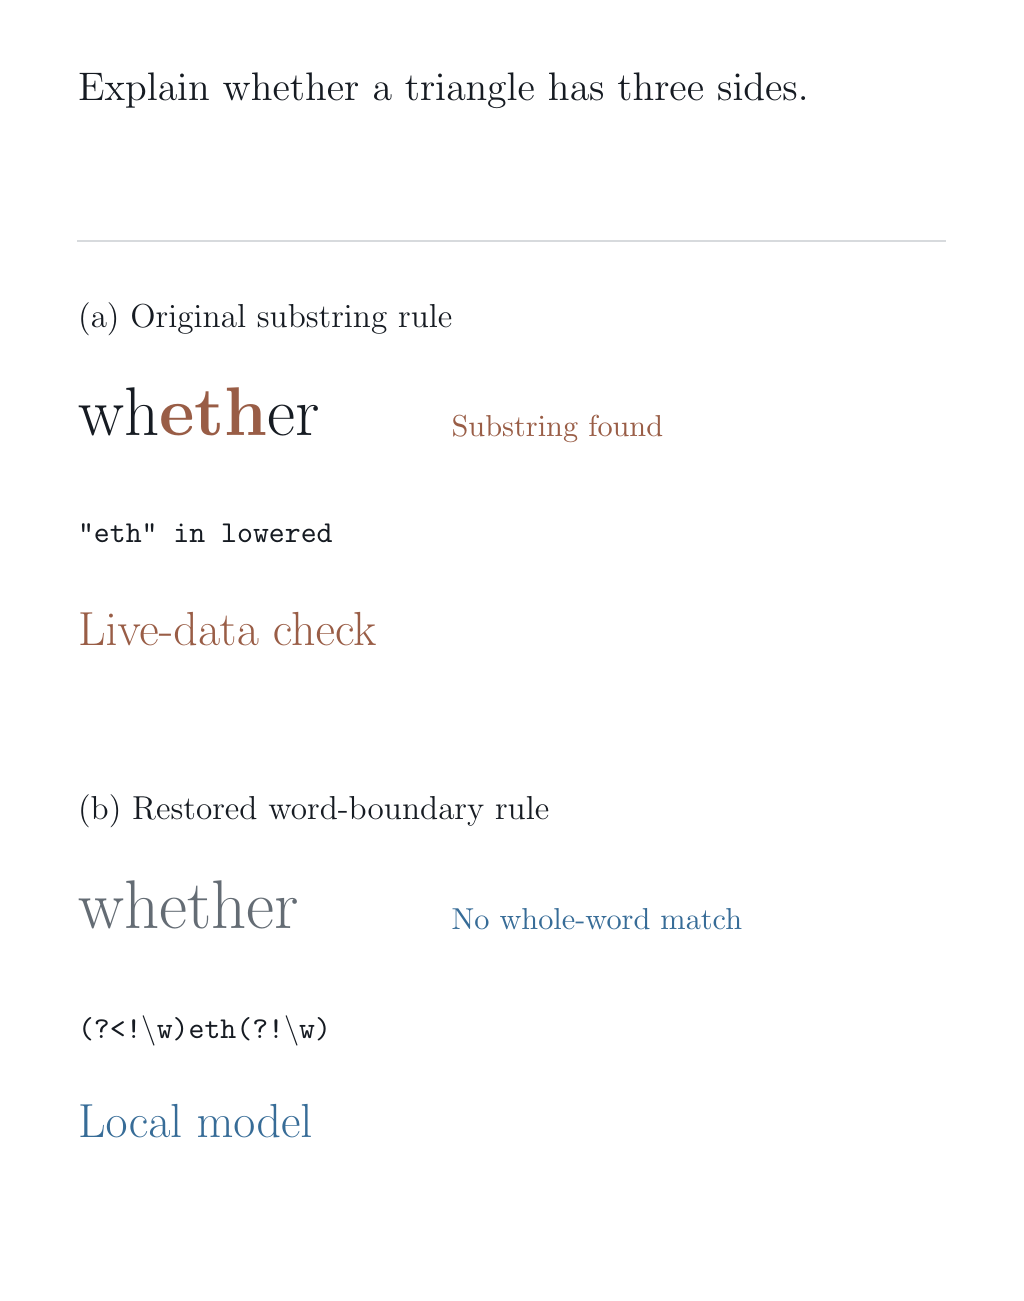
\begin{tikzpicture}[x=1pt,y=-1pt]
\path[use as bounding box] (0,0) rectangle (350,450);
\node[anchor=north west,inner sep=0pt,text=ink,align=left,font=\fontsize{14}{21.0}\selectfont,text width=314pt] at (18,16) {Explain whether a triangle has three sides.};
\draw[line,line width=.6pt] (18,77) -- (332,77);
\node[anchor=north west,inner sep=0pt,text=ink,align=left,font=\fontsize{12}{18.0}\selectfont] at (18,99) {(a) Original substring rule};
\node[anchor=north west,inner sep=0pt,text=ink,align=left,font=\fontsize{24}{36.0}\selectfont] at (18,130) {wh\textcolor{api}{\textbf{eth}}er};
\node[anchor=north west,inner sep=0pt,text=api,align=left,font=\fontsize{11}{16.5}\selectfont] at (153,140) {Substring found};
\node[anchor=north west,inner sep=0pt,text=ink,align=left,font=\fontsize{10.8}{16.200000000000003}\selectfont] at (18,179) {\texttt{"eth" in lowered}};
\node[anchor=north west,inner sep=0pt,text=api,align=left,font=\fontsize{18}{27.0}\selectfont] at (18,211) {Live-data check};
\node[anchor=north west,inner sep=0pt,text=ink,align=left,font=\fontsize{12}{18.0}\selectfont] at (18,277) {(b) Restored word-boundary rule};
\node[anchor=north west,inner sep=0pt,text=ink,align=left,font=\fontsize{24}{36.0}\selectfont] at (18,308) {\textcolor{muted}{whether}};
\node[anchor=north west,inner sep=0pt,text=local,align=left,font=\fontsize{11}{16.5}\selectfont] at (153,318) {No whole-word match};
\node[anchor=north west,inner sep=0pt,text=ink,align=left,font=\fontsize{10.8}{16.200000000000003}\selectfont] at (18,357) {\texttt{(?<!\textbackslash w)eth(?!\textbackslash w)}};
\node[anchor=north west,inner sep=0pt,text=local,align=left,font=\fontsize{18}{27.0}\selectfont] at (18,389) {Local model};

\end{tikzpicture}
\end{document}
